\documentclass[a4paper,10pt]{report}
\usepackage[utf8]{inputenc}
\usepackage[frenchb]{babel}
\usepackage{fancyhdr}
\usepackage{graphicx}
\usepackage{multicol}
\usepackage{array}
\usepackage{float}
\usepackage{chngcntr}


\pagestyle{fancy}
\renewcommand\headrulewidth{0pt}
\renewcommand\footrulewidth{1pt}
\fancyfoot[L]{Projet STCal}
\fancyfoot[R]{IUT Informatique de Belfort}
\lhead{}
\rhead{}
\date{}
\makeatletter
\let\ps@plain=\ps@fancy
\makeatother


\renewcommand{\chaptername}{}

\title{\Huge{Projet STCal}\\ {\Large Rapport général}}
\author{Florian Barrois \and Nicolas Devilers \and Valentin Jeanroy \and Mehdi Loisel \and Jean Mercadier \and Ismail Taleb \and Willeme Verdeaux}


\begin{document}
 \begin{titlepage}

\begin{center}
~\\~\\~\\~\\~\\
\Huge
Projet STCal\\
\LARGE
Rapport général\\
~\\~\\~\\~\\~\\~\\
\begin{multicols}{3}
\large
Florian Barrois\\Mehdi Loisel\\
\columnbreak 
Nicolas Devilers\\Jean Mercadier\\Willeme Verdeaux\\
\columnbreak
Valentin Jeanroy\\Ismail Taleb
\end{multicols}
\end{center}


\begin{center}
~\\~\\~\\~\\~\\~\\~\\~\\~\\~\\~\\~\\
 
\includegraphics{iutbm.jpeg}
 ~\\~\\~\\~\\~\\
\large
Année 2013-2014
\end{center}

\end{titlepage}

\strut
\renewcommand{\contentsname}{Sommaire}
\tableofcontents

\part{Introduction}
  \paragraph{}
    Le projet que nous nous apprêtons à vous présenter est celui réalisé par notre groupe de sept étudiants suivant des cours en informatique à l'Institut Universitaire de Belfort.
    
  \paragraph{}
    Dans le cadre de notre projet tutoré, nous avons dû réfléchir à un secteur d'activité nécessitant des outils informatiques relativement simples mais essentiels. 
    Ainsi, au vu du besoin éprouvé par nos enseignants de travailler avec des outils plus simples, nous avons choisi de réaliser un progiciel à utilité pédagogique.
    Cette application aura pour but de faciliter la gestion des stages des étudiants de quatrième semestre ainsi que la mise en place d'un calendrier des soutenances orales des étudiants présentant leur stage à leurs professeurs.

  \paragraph{}
    L'application possédera bien sûr des fonctionnalités précises, correspondant aux besoins des enseignants s'occupant des stages, mais ces fonctionnalités seront également conçues de manière à ce que la plupart des établissements d'enseignement supérieur et des organismes gérant des stages puissent s'en servir de façon intuitive. 
    Poursuivant l'objectif de produire un travail complet tout en se mettant dans la peau des utilisateurs, les moyens les plus modernes et adaptés, du point de vue technique, et les plus faciles d'utilisation, du côté de l'usager, seront mis en place pour satisfaire au maximum la demande concernant l'organisation de stages. 

  \paragraph{}
    Nous détaillerons ainsi dans ce rapport toute notre réflexion pour répondre à cette problématique, expliquerons nos choix, et parlerons des avantages et des éventuels inconvénients liés à ces derniers.  
    Des illustrations seront également placées tout au long du rapport dans le but d'apporter une meilleure compréhension et une représentation concrète du travail réalisé.
    
  \paragraph{}
    Nous allons donc étudier les différents aspects du projet, en commançant par une brève présentation du sujet. 
    Puis nous nous tournerons vers le cahier des charges, qui comprendra les fonctionnalités du produit ainsi que les contraintes à respecter.
    Ensuite, nous observerons plus en détail comment s'est déroulée la réalisation des différentes étapes.
    Enfin nous aborderons les difficultés survenues et concluerons sur le résultat obtenu et sur le projet en lui-même.



\part{Présentation du sujet}
  \paragraph{}
    Depuis de nombreuses années, les professeurs de notre établissement, et sûrement bien d'autres, s'occupent des stages en s'adaptant aux outils existants.
    En effet, à ce jour, la méthode employée pour réaliser cette tâche se compose de la gestion d'une part des informations, et d'autre part du planning des soutenances, en utilisant respectivement des logiciels tels que Microsoft Excel, et les fonctionnalités de calendrier de Google.
    La mission dont nous nous sommes acquittés consiste donc à aider les responsables de stage, non pas par la recherche d'outils plus appropriés, mais par la création d'une application qui sera spécifiquement prévue à cet usage et qui demeurera parfaitement adaptée aux besoins des usagers, notamment du personnel enseignant.

  \paragraph{}
    Ainsi la difficulté de ce défi est conséquente, puisque nous ne connaissons aucun outil similaire existant pouvant servir de référence ou permettant d'étayer notre réflexion.
    Notre groupe de sept étudiants a donc été chargé de trouver la bonne démarche à suivre en mettant à profit toutes les connaissances, qu'elles aient été acquises en cours ou à la suite de recherches liées au projet.
    Les connaissances utilisées relèvent de la mise en place d'une interface graphique, de la gestion de classes et de bases de données, en plus de toutes les notions apprises liées au langage utilisé, à savoir le Java.
  
  \paragraph{}
    Le résultat ne consistera en aucun cas en une plate-forme de consultation des stages.
    L'application développée sera mise à disposition exclusive des enseignants et du personnel responsable des stages. 
    Les étudiants concernés n'auront quant à eux aucun accès à l'application, que ce soit pour ajouter, supprimer, consulter ou éditer des données.
    
    
    
\part{Cahier des charges}
  
  \chapter{Fonctionnalités}

    L'application Stcal devra simplifier la gestion des stages des étudiants par les professeurs grâce à plusieurs fonctionnalités, réparties ci-dessous en quatre étapes  :

    \begin{enumerate}
      \item La création de stages.
      \item La création et la gestion d’un emploi du temps.
      \item La création d'une base de données. 
      \item L'existence d'un système de sauvegarde.
    \end{enumerate}
  ~\\~\\
    \paragraph{}
      En plus de ces quatre fonctions principales, d'autres seront créées dans le but de faciliter le travail de l'utilisateur. 
  

  \chapter{Développement et contraintes}

    Le développement s'effectuera en quatre étapes, qui contiendront les différentes tâches. Ces étapes et tâches seront ordonnées de manière à ce que le côté fonctionnel de l'application soit prioritaire :

    \section{Première étape}

      \subsection{Développement}
	\paragraph{}
	L'application devra avant tout considérer des étudiants et des professeurs.
	\newline
	Le produit permettra ainsi l'import de fichiers contenant les données. 
	Ces dernières seront par la suite utilisées lors de la création de couples professeur/étudiant. 
  
      \subsection{Contraintes}
	\paragraph{}
	Détaillons maintenant les différentes contraintes à respecter concernant cette étape. 
	\paragraph{}
	A partir d'une liste de professeurs et d'une liste d'étudiants existantes, un bouton devra permettre d'associer un étudiant à un professeur.
	N'ayant qu'un tuteur de stage, chaque étudiant sera relié à un et un seul enseignant.
	En revanche, un enseignant peut posséder la fonction de responsable de stages pour plusieurs élèves. 
	Chaque enseignant pourra donc être relié à aucun, un ou plusieurs étudiants.	
	
      
	
    \section{Deuxième étape}

      \subsection{Développement}
	
	\paragraph{}
	L’application comportera une fonction de création d’emploi du temps vide et une seconde permettant le remplissage de celui-ci avec les soutenances de chacun des étudiants.
	\newline
	\newline
	Les plages horaires réservées contiendront les informations suivantes :
	\newline
	\renewcommand\labelitemi{\textbullet}
	\begin{itemize}
	  \item Le nom de l’enseignant tuteur;
	  \item Le nom de l’enseignant candide ;
	  \item Le nom de l’étudiant;
	  \item Le numéro de la salle d’entretien.
	\end{itemize}
	
	\paragraph{}
	Le progiciel possédera également une option d’export du calendrier généré au format ICS compatible avec Google et iCal.
	
      \subsection{Contraintes}
	\paragraph{}

	Le produit devra être capable de résoudre les cas suivants en affichant un message d’erreur et en ignorant la dernière action effectuée :
	\newline
	\renewcommand\labelitemi{\textbullet}
	\begin{itemize}
	  \item en cas de création d'une soutenance à un horaire incompatible pour l'enseignant tuteur ;
	  \item en cas de création d'une soutenance à un horaire incompatible pour l'enseignant candide ;
	  \item en cas de création d'une soutenance ayant lieu dans une salle déjà réquisitionnée à cet horaire ;
	  \item si toutes les salles d’entretien venaient à être occupées à un horaire donné, cette plage horaire devra être inaccessible pour placer d’autres soutenances.
	\end{itemize}
  
      

    \section{Troisième étape}
      \subsection{Développement}
	\paragraph{}
	Le produit possédera un outil de création de base de données dans laquelle les stages pourront être stockés. 
	Les informations enregistrées seront identiques à celles affichées sur les horaires de soutenances. 
	La base de données créée pourra ensuite être reliée à un client léger, comme un site web dynamique, et sera consultable par les étudiants.

      \subsection{Contraintes}
	\paragraph{}
	  La contrainte principale de cette étape consiste à éviter la présence de doublons dans la base données. 
	  Le progiciel devra donc afficher un message d'erreur si les données telles que le nom et le prénom d'une personne, étudiant ou enseignant, entrées dans l'application sont déjà présentes dans la base de données. 
      
      ~\\~\\~\\~\\
      
    \section{Quatrième étape}
      \subsection{Développement}
	\paragraph{}
	  L’application contiendra un système de sauvegarde : lors de l’ouverture de l’application par l’utilisateur, le système effectuera une restauration de session qui permettra l’affichage de la dernière page affichée avant la fermeture de l’application lors la session de travail précédente.

      \subsection{Contraintes}
	\paragraph{}
	  Lors de la première utilisation du progiciel, l'utilisateur devra entrer les paramètres correspondant à la base de données qui stockera les informations, à savoir le nom du serveur, le port utilisé, le nom d'utilisateur et le mot de passe.
	  Une fois les champs renseignés, ces paramètres seront également mémorisés et la restauration de session devra passer par un accès cette base de données pour afficher les informations précédemment enregistrées.
	  Le programme sera donc contraint de rechercher l'existence d'un fichier de configuration dans l'ordinateur afin de savoir si l'application est utilisée ou non pour la première fois.
	  Si c'est le cas, une fenêtre contenant les différents paramètres à renseigner mentionnés précédemment apparaît, et les valeurs entrées sont mémorisées dans un nouveau fichier de configuration.
	  ~\\
	  ~\\
	  ~\\
	  ~\\
	  ~\\
	\paragraph{}
	  Ces étapes consistuent ainsi le fil conducteur du projet. 
	  Il faut également noter l'existence d'une autre étape effectuée en parallèle : la réalisation de l'interface graphique.
	  En effet, celle-ci offre la possibilité d'entrevoir le rendu final qui sera livré au client et facilite également la visibilité quant à l'évolution du projet.
	  Elle permet aussi d'incorporer directement dans le progiciel les fonctions programmées en interne au fur et à mesure que le projet progresse et tient ainsi le rôle de de plate-forme de tests.   
	
\part{Réalisation}
  \setcounter{chapter}{0}
  \counterwithout{figure}{chapter}
  
	\paragraph{}
	  Nous avons abordé la problématique et les étapes du sujet.
	  Quittons maintenant la théorie et les prévisions pour entrer dans le concret.
	  Cette partie va détailler la réalisation effective du projet.
	  Les quatre étapes principales, ainsi que celle concernant l'interface graphique, vont pouvoir être rattachées à un véritable support.
	  
	\paragraph{}
	  Les futurs utilisateurs du produit seront relativement nombreux, par conséquent les systèmes d'exploitation peuvent varier, avec notamment Windows, connu et employé couramment par une grande communauté de personnes, Linux, qui est très utilisé dans le cadre de nos études, et Mac OS, qui devient de plus en plus répandu.
	  C'est pourquoi toute l'application sera programmée en Java, ce qui permettra l'usage du progiciel sous n'importe quelle plate-forme et favorisera une programmation orientée objet.
	  Tout au long de cette partie, les outils auxquels nous avons fait appel et qui seront mentionnés se trouveront donc être des fonctions et des objets instanciés en Java.
	  Quant à l'interface graphique, elle sera implémentée à partir la bibliothèque graphique Java Swing.
  
  
  \chapter{Interface}
	\paragraph{}
	  L'interface de l'application contient une barre de menu donnant accès aux multiples possibilités offertes par l'application.
	  Le corps de l'interface affiche quant à lui trois onglets principaux dédiés aux différentes fonctionnalités du progiciel. 
	  
	\section{Le menu}
	
	  \paragraph{}
	    La barre de menu est composée elle-même de plusieurs sous menus.
	  \paragraph{}
	    Le premier sous menu est intitulé ``Fichier``. Il offre la possibilité d'importer une liste d'étudiants et une liste de professeurs depuis un fichier au format CSV.
	    En cas de problème avec le fichier à importer, l'application le signale bien évidemment à l'utilisateur par le biais d'une popup d'erreur et annule l'import.
	    Il présente également une fonction d'export, notamment pour le calendrier généré. Cette fonction exporte le planning des soutenances au format PDF, ou encore ICS, qui permet la compatibilité avec les calendriers Google notamment.
	    La dernière option de ce menu sert à fermer l'application.
	  \paragraph{}
	    Le deuxième sous menu a pour libellé ''Actions``, et propose de lier un étudiant à un enseignant. 
	    Cette fonctionnalité ne fonctionne que si l'utilisateur a auparavant sélectionné l'étudiant et l'enseignant concernés.
	  \paragraph{}
	    Le troisième champ est nommé ''Préférences``.
	    Il est dédié au côté Base de Données du programme.
	    Un de ses onglets possède le libellé ''Base de données`` et ouvre une fenêtre permettant à l'utilisateur de mettre à jour les paramètres de la base de données énumérés dans la quatrième étape du cahier des charges. 
	    Un autre onglet donne l'opportunité de réinitialiser la connexion à la base de données correspondant aux paramètres en vigueur.
	    Un dernier lien permet de modifier la liste des salles de présentation des soutenances. 
	    L'utilisateur peut notamment ajouter de nouvelles salles dans la liste et en supprimer.
	  \paragraph{}
	    La quatrième et dernière rubrique propose un champ ''Aide``, qui affiche le manuel d'utilisateur.
	    Elle présente également un champ qui redirige l'usager vers une brève présentation du projet STCal. 

	    
        \section{Les onglets}
	  
	  \paragraph{}
	    Trois onglets sont accessibles à l'utilisateur.
	  
	  \paragraph{L'onglet Lier}
	  ~\\~\\
	  
	    \begin{figure}[!h]
	  
	    \hbox to12cm{\hss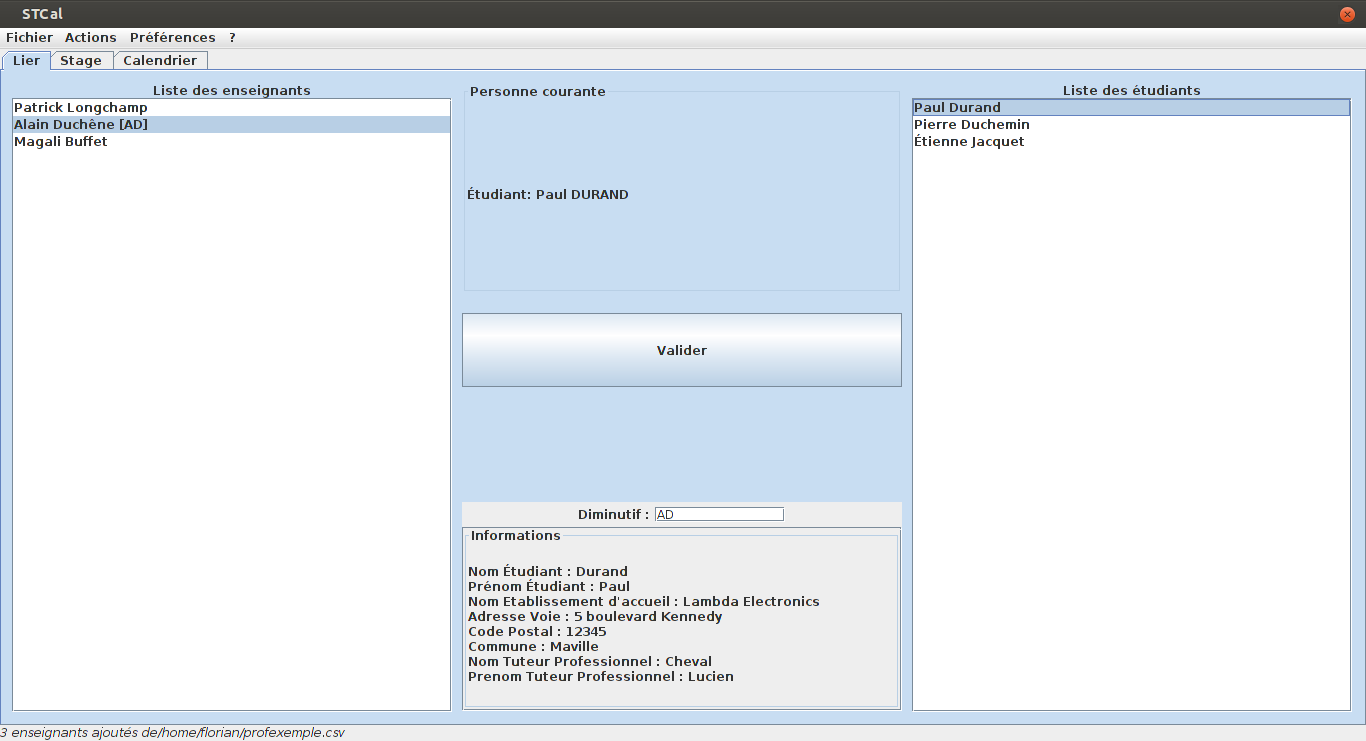
\includegraphics[width=18cm]{Lier.png}\hss}
	    \caption{Onglet Lier après imports}
	    \end{figure}

	  
	  
	    \paragraph{}
	      La première page est destinée à afficher les acteurs principaux, à savoir les étudiants et les enseignants. 
	      En effet, on peut diviser cette page intitulée ''Lier`` en trois parties.
	      
	    \paragraph{}
	      La partie de gauche affiche une liste de professeurs importée depuis un fichier CSV, et de la même manière, la partie de droite montre une liste d'étudiants provenant d'un deuxième fichier au format CSV.
	      Les personnes, étudiants et enseignants, contenues dans ces listes ne sont alors caractérisées que par leur nom et leur prénom.
	      Il faut bien noter que l'import est obligatoire puisque l'application ne possède aucune fonctionnalité d'établissement de listes.
	    
	    \paragraph{}
	      La partie centrale contient les appels aux fonctions nécessaires à l'import des fichiers d'étudiants d'une part, et à l'import des fichiers d'enseignants d'autre part.
	      Ces fonctions demeurent accessibles grâce à des boutons portant le libellé correspondant.
	     
	    \paragraph{}  
	      Ces boutons ne sont disponibles qu'une fois chacun : après l'import d'un fichier d'étudiants, respectivement d'enseignants, le bouton consacré à cette tâche n'est plus présent.
	      Toutefois, il reste possible de réaliser de nouveaux imports à partir de la barre de menu située en haut de l'interface de l'application.
	      Les personnes précédemment affichées dans la liste des objets du type de l'import immédiatement effectué sont alors remplacées par les valeurs du nouveau fichier.  
	      
	    \paragraph{}      
	      La zone centrale présente également une portion révélant le statut et les nom et prénom de la dernière personne sélectionnée.
	      Un autre cadre situé en bas de la fenêtre affiche aussi toutes les informations complémentaires connues au sujet de la personne sélectionnée, comme le numéro de téléphone, ou l'adresse par exemple.
	      Au-dessus ce ce cadre se trouve un champ permettant la saisie d'un diminutif pour professeur sélectionné.
	      Ce champ est en revanche inaccessible à la saisie de diminutif d'un étudiant.      
	      Une fois un étudiant et un professeur sélectionnés, un bouton de validation apparaît.
	      Ce bouton peut être actionné seulement si un étudiant et un professeur auquel a été attribué un diminutif sont sélectionnés.
	    
	    \paragraph{}
	      Après avoir enclenché ce bouton, les identifiants de la dernière personne sélectionnée disparaissent pour laisser place à la phrase de confirmation ''Stage créé``.
	      En effet, on considérera comme stages les couples étudiant/enseignant effectués.
	      Un stage est alors formé et consultable dans l'onglet ''Stages``. 
	      L'étudiant concerné est alors effacé de la liste, en revanche, le professeur conserve sa disponibilité pour s'occuper des stages d'autres étudiants.
	      Aucun étudiant n'étant alors sélectionné, le bouton de validation reste inaccessible jusqu'à ce qu'un enseignant et un nouvel étudiant soient sélectionnés.
	      
	      \newpage
	  \paragraph{L'onglet Stage}
	  ~\\~\\
	      \begin{figure}[H]
		\hbox to12cm{\hss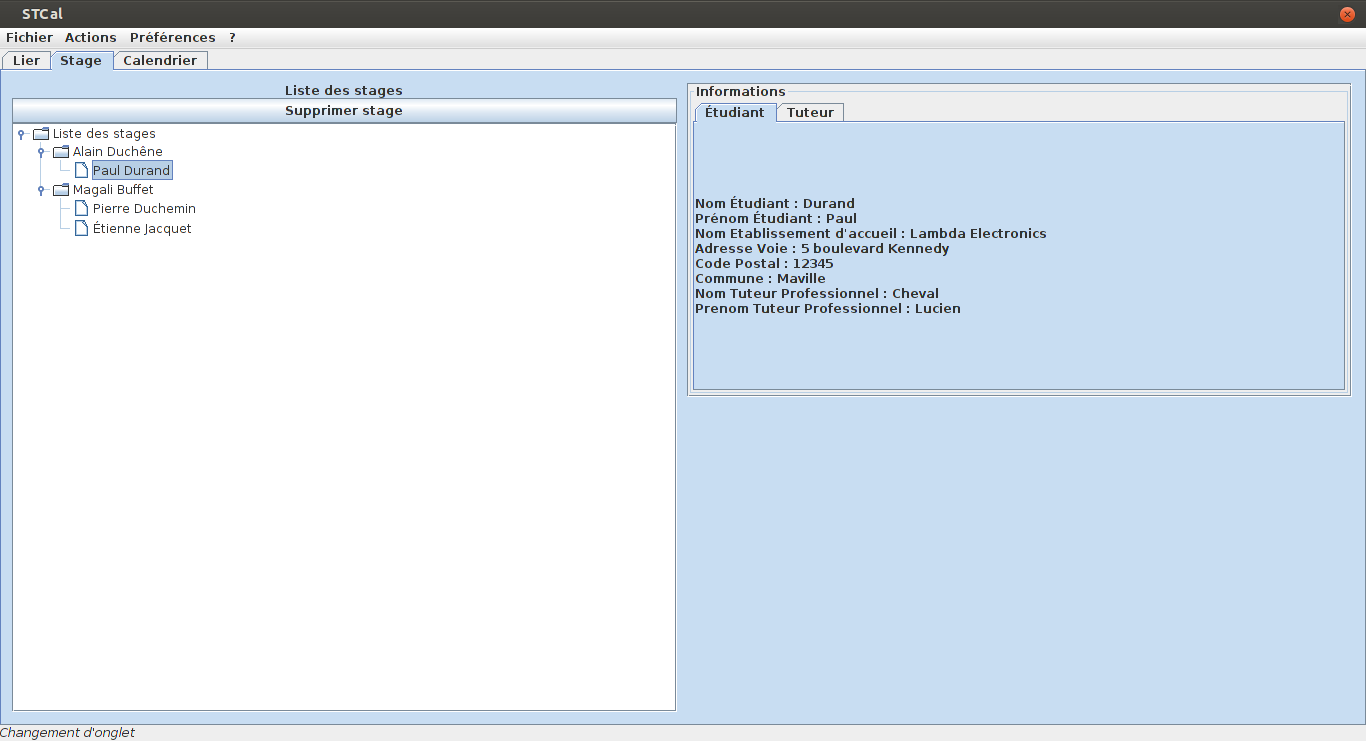
\includegraphics[width=18cm]{Stage.png}\hss}
		\caption{Onglet Stage}
	      \end{figure}
	  
	 
	      \paragraph{}
		L'onglet ''Stage`` contient également deux sections.
		
		
		
	      \paragraph{}
		La partie gauche est consacrée à l'affichage des différents stages créés dans l'onglet précédent.
		Cette affichage est présenté sous forme d'arborescence.
		Le dossier racine a pour titre ''Listes des stages``.
		Il contient alors plusieurs sous-dossiers correspondant aux professeurs liés à au moins un étudiant.
		Ces sous-dossiers possèdent des fichiers représentant les étudiants liés à l'enseignant en question.
		
	      \paragraph{}
		Dans cette moitié gauche se trouve également un bouton permettant la suppression d'un stage.
		Ce bouton est accessible uniquement dans le cas où un étudiant est sélectionné.
		Les dossiers-professeurs ainsi que le dossier racine ne peuvent être supprimés.
		La dossier racine est donc toujours présent dans cette section.
		Un dossier, représentant un professeur ne disparaît que lorsqu'il ne contient aucun étudiant.
		Ainsi, en cas de suppression du dernier stagiaire rattaché à un enseignant, le dossier symbolisant ce dernier disparaît en même temps que le fichier-étudiant.
		De cette manière, un dossier n'est jamais vide.
		
	      \paragraph{}
		Lorsqu'un étudiant est supprimé de cette arborescence, le stage est effacé.
		L'étudiant réapparaît alors dans la liste de tous les étudiants située dans l'onglet ''Lier`` et redevient disponible pour une affectation à un professeur.
		
	      \paragraph{}
		La moitié droite de cette fenêtre renseigne avec plus de détails sur les personnes présentes dans l'arborescence représentant les stages.
		En effet, on peut remarquer la présence d'un cadre appelé ''Informations``, qui contient lui-même deux fenêtres.
		La première est vouée à détailler les informations de l'étudiant courant. 
		Quant à la seconde, elle renseigne l'utilisateur sur les données se rapportant au professeur en charge du stage de l'étudiant courant. 
		Cette moitié de l'onglet ''Stage`` expose également une phrase d'indication de la démarche à suivre pour connaître les données approfondies d'une personne, destinée au client lors de sa première venue sur cet onglet.
		
		\newpage
	    \paragraph{L'onglet Calendrier}
	      \paragraph{}
		\textit{Dans cette partie, il importe de savoir que du point de vue de la hiérarchie des classes gérant le calendrier, on considère qu'une journée est divisée en créneaux, qui correspondent aux horaires de passage, contenant eux-mêmes des soutenances, qui sont caractérisées par un couple étudiant/professeur et une salle	.} 
		
		\begin{figure}[!h]
		\hbox to12cm{\hss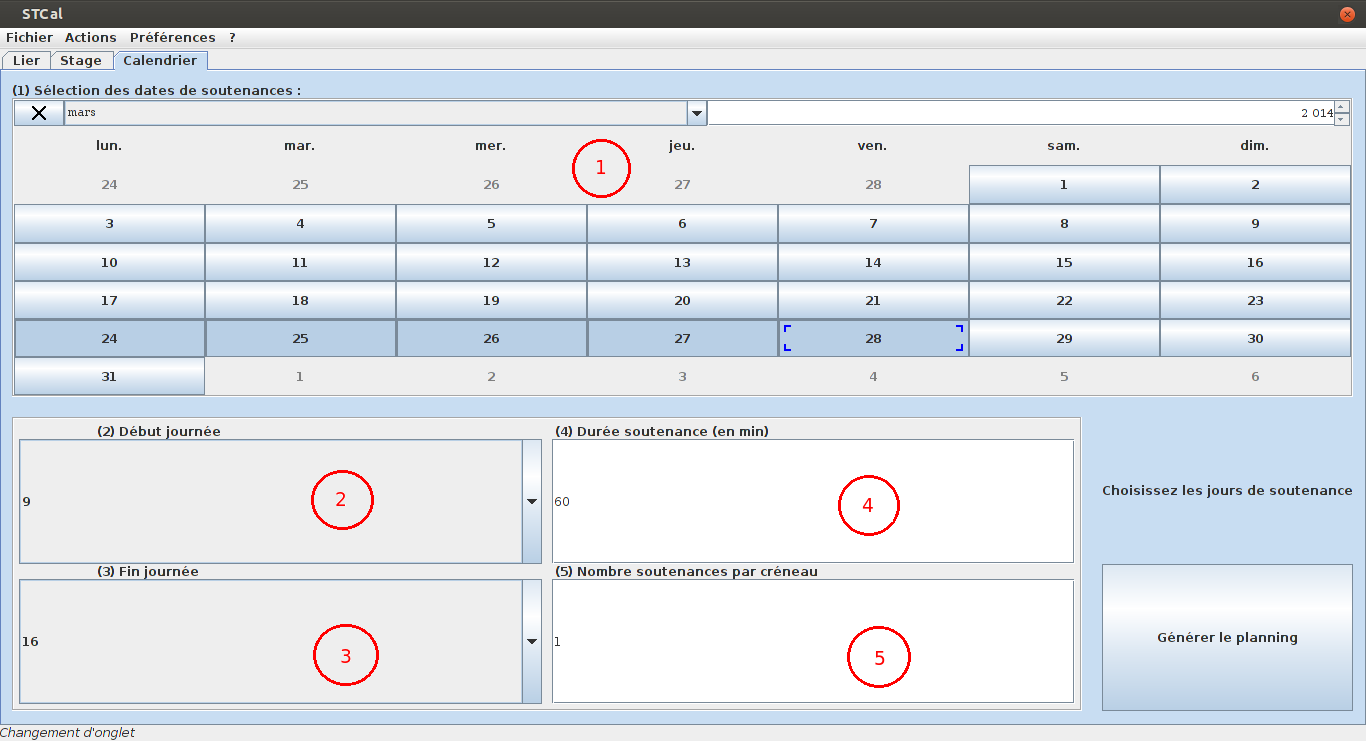
\includegraphics[width=18cm]{Calendrier.png}\hss}
		\caption{Onglet de paramètrage du calendrier}
		\end{figure}
		
	      \paragraph{}  
		La création d'un calendrier nécessite plusieurs étapes préliminaires.
		En effet, l'usager doit passer par le renseignement de cinq paramètres avant de pouvoir générer un planning de soutenances.
		
	      \paragraph{}
		L'interface de cet onglet est scindé horizontalement en deux zones.
		La zone du haut est uniquement vouée à la première information à définir.
		Il s'agit de la date de la soutenance.
		Un calendrier occupe donc l'espace supérieur de l'interface.
		Chaque case du calendrier est cliquable, l'utilisateur choisit donc le jour qu'il souhaite par ce moyen.
		Il peut bien sûr régler le mois et l'année grâce à des champs situés juste au dessus du calendrier.
		Par défaut, la date choisie est la date courante.
		
	      \paragraph{}
		La zone inférieure de cet onglet du progiciel concerne tous les autres paramètres à déterminer.
		Une fois la date choisie, l'usager doit choisir les heures de début et de fin de la journée.
		Deux champs sont alors mis à sa disposition sous forme de listes déroulantes contenant toutes les heures entières de 7h à 20h.
		Après avoir fixé la date de début de journée, la deuxième liste déroulante ne possède évidemment plus que les heures postérieures à la date de début.
		
	      \paragraph{}
		La prochaine étape consiste à établir la durée d'une soutenance.
		Enfin, le responsable de stages doit saisir le nombre de soutenances maximal qu'il est possible d'organiser à un même horaire.
		Tous les champs étant remplis, le planning peut alors être généré.
		~\\~\\
		
		\begin{figure}[!h]
		\hbox to12cm{\hss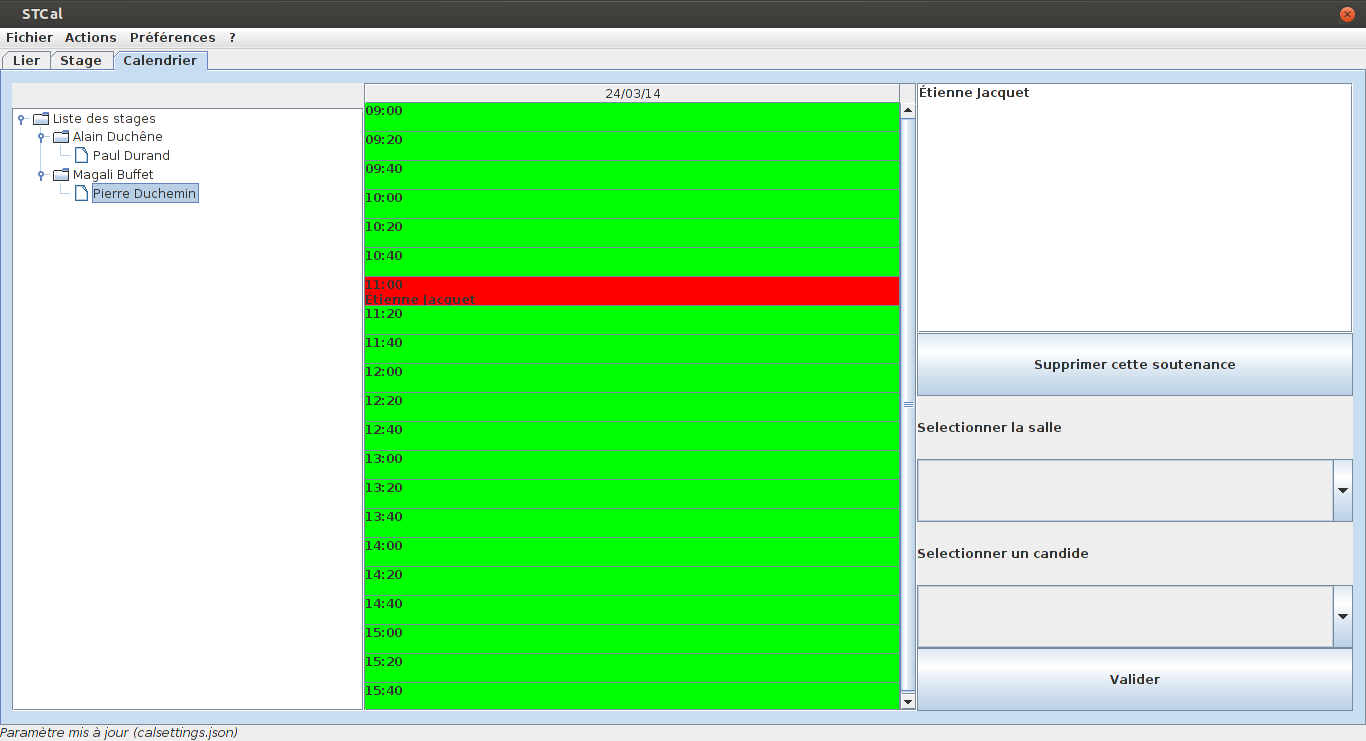
\includegraphics[width=18cm]{Calendrier2.png}\hss}
		\caption{Onglet Calendrier}
		\end{figure}
		
	      \paragraph{}
		Lorsque la fonction de génération du calendrier est enclenchée, une redirection est effectuée vers une nouvelle page.
		Cette dernière présente une zone dans laquelle sont affichés les noms des étudiants faisant partie d'un stage, une deuxième affichant le planning de la journée choisie précédemment, et une troisième énumérant les étudiants passant leur soutenance à un horaire préalablement sélectionné.
		
	      \paragraph{}
		La première section montre uniquement les étudiants étant rattachés à un responsable de stage, composant ainsi un stage.
		On retrouve alors l'arborescence présente dans l'onglet précédent.
		
	      \paragraph{}
		La partie centrale affiche tous les horaires de la journée sélectionnée pour les soutenances.
		La date est écrite en haut de ce planning.
		Les horaires de passage dépendent logiquement de la durée d'une soutenance.
		Les soutenances sont créées simplement par déplacement d'un étudiant sur un créneau.
		Dès qu'un étudiant est sélectionné, les créneaux changent de couleur : les créneaux de couleur verte sont disponibles pour la soutenance de cet étudiant.
		A l'inverse, si un créneau est devient rouge, il demeure inaccessible pour ce stage.
		Les modalités d'indisponibilité d'un créneau sont celles spécifiées dans la deuxième partie du cahier des charges.
		En cas de tentative de création d'une soutenance à une plage horaire bloquée, un message expliquant la nature du problème apparaît.
		
	      \paragraph{}
		A la création d'une soutenance, le nom de l'étudiant s'inscrit dans le créneau, à côté de l'heure à laquelle débute celui-ci.
		Lorsqu'une plage est sélectionnée, l'étudiant apparaît également dans la troisième partie de la page située dans le tiers le plus à droite, qui révèle sous forme de liste tous les étudiants passant leur examen oral à cet horaire.
		En cliquant sur un des éléments de cette liste , toutes les informations relatives à la soutenance de cet étudiant, à savoir le tuteur, l'enseignant candide et la salle de la soutenance, apparaissent dans le coin inférieur gauche de l'écran.
		Le troisième tiers de la page propose également les fonctionnalités permettant d'ajouter un enseignant candide et une salle à une soutenance, ceci par le biais de deux listes déroulantes listant respectivement les enseignants et les salles disponibles à cet horaire.
		Les salles seront à créer au préalable depuis l'onglet ''Préférences`` de la barre de menu.
		
	      \paragraph{}
		Un bouton de suppression d'une soutenance est présent en bas dessous de la listes des soutenances pour un créneau.
		La fonction liée à ce bouton permet d'effacer une soutenance sans effacer le stage.
		C'est pourquoi l'étudiant en question disparaît du créneau et de la liste de droite mais reste visible dans la liste de gauche et dans l'onglet ''Stage``, qui demeure ainsi l'unique onglet dans lequel supprimer un stage est possible.
		
		~\\
		~\\
		~\\
		~\\
		~\\
	      \paragraph{}
		Comme nous avons pu le remarquer, la réalisation demeure assez complète.
		De plus, l'interface est hiérarchisée et aérée, ce qui fait de l'application un outil très simple d'utilisation, et ce même pour les personnes mal à l'aise avec l'informatique.
		
  \chapter{Données}
      \paragraph{}
	Après cette partie finalement essentiellement orientée vers l'apparence de l'application, nous allons poursuivre en expliquant le mode de fonctionnement de notre code et faire le point sur les outils utilisés en opposant les fonctions déjà existantes à celles créées par nos soins.
		   
    \section{Mode de fonctionnement}
      \paragraph{}
	Poursuivant l'idée de travailler un code clair, bien ordonné et facilement accessible, nous avons opté pour une hiérarchie de nos classes basée sur la forme Modèle-Vue-Contrôleur.
	Ainsi, il nous est enfantin d'isoler les parties à conserver ou modifier en déterminant simplement si les parties fonctionnelles, ou les problèmes, viennent des données, de leur traitement ou de leur affichage.
      
      \paragraph{}
	Les classes Java ne seront pas détaillées dans ce rapport car leur description sera l'objet d'un rapport technique.
	A titre d'indication rapide notons simplement que les classes essentielles sont celles permettant d'instancier un étudiant, un professeur et un couple réunissant ces deux propriétés.
	La quasi totalité des autres classes concernant le modèle et le contrôleur sont donc issues de ces dernières et possèdent généralement des relations d'héritage avec celles-ci, ce qui permet le traitement des données dans toute l'application.
	Le même principe d'héritage est appliqué aux classes de gestion du calendrier, un créneau étant composé de soutenances, elles-mêmes réunissant un stage et un enseignant candide.
	
	
	
    \section{Outils}
      \paragraph{}
	Ce projet a été le fruit résultant de l'union de nos créations et d'outils déjà existants. 
	En effet, l'application été destinée à une utilisation pour un domaine bien précis, et n'ayant jamais connu de prototype par le passé, toutes les classes et méthodes de nos codes sources ont été entièrement réalisées durant cette année par notre groupe.
	Tous les programmes spécifiques aux stages, c'est-à-dire la majorité, relèvent donc de notre accomplissement.
	Mais une partie du projet a néanmoins été réalisée à partir de méthodes existantes. 
	Il s'agit notamment de la partie graphique, pour laquelle la bibliothèque Swing a été contributive par le biais de widgets et de layouts tels que \textit{JPanel}, \textit{JScrollPane} ou encore \textit{ActionListener}.
	
	
		
\part{Gestion du projet}
\setcounter{chapter}{0}
\counterwithout{figure}{chapter}
      \paragraph{}
	  La réalisation de notre progiciel est au final plutôt aboutie, mais comme dans tout projet, chacun des membres de notre groupe a connu des difficultés, qui se sont présentées sous différentes formes.
	  ~\\~\\
	  Voyons ensemble, quelles ont été ces dernières à travers la répartition des tâches, la gestion du temps et les difficultés liées au travail en lui-même.
	
  \chapter{Répartition des tâches}
    \paragraph{}
      La répartition des différents tâches a été effectuée comme indiquée ci-après.
      Nous avons fait en sorte que chacun travaille sur toutes les parties du projet, ce qui nous a permis à la fois d'approfondir et de diversifier nos connaissances.

      \begin{figure}[H]
	\hbox to12cm{\hss
	  \begin{tabular}{|l|l|}
	    \hline
	    \textbf{Membres du groupe} & \textbf{Tâches effectuées} \\
	    \hline
	      Florian Barrois 
	      & Réalisation des classes de base du modèle (Étudiant, Professeur, Couple...); \\
	      & Conception du modèle; \\
	      & Mise en fonctionnement de certaines fonctionnalités de la barre de menu;\\
	      & Optimisation de l'interface;\\
	      & Rédaction du rapport général et du manuel d'utilisateur.\\
	    \hline
	      Nicolas Devilers 
	      & Gestion des classes permettant l'import de fichiers CSV;\\
	      & Optimisation de l'interface.\\
	      \hline
	      Valentin Jeanroy 
	      & Conception du modèle et implémentation de celui-ci sur toutes les classes; \\
	      & Travail réalisé sur l'interface;\\
	      & Mise en place du fonctionnement et de l'interface du calendrier;\\
	      & Travail réalisé sur l'export de fichiers;\\
	      & Gestion des listes et arborescences.\\
	      \hline
	      Mehdi Loisel 
	      & Mise en place du fonctionnement et de l'interface du calendrier; \\
	      & Gestion de l'export de calendrier au format ICS;\\
	      & Travail réalisé sur l'interface;\\
	      & Optimisation de l'interface;\\
	      & Gestion d'ajout de l'enseignant candide et de la salle;\\
	      & Travail réalisé sur l'export de fichiers.\\
	      \hline
	      Jean Mercadier
	      & Création de l'interface; \\
	      (chef de projet)& Travail réalisé sur l'interface et les retours en console;\\
	      & Mise en fonctionnement de certaines rubriques de la barre de menu;\\
	      & Rédaction de la plupart des fichiers et du programme principal;\\
	      & Implémentation de la base de données;\\
	      & Création des fichiers d'importation;\\
	      & Rédaction du rapport technique.\\
	      \hline
	      Ismail Taleb 
	      & Mise en place de la fonctionnalité de ''Drag and Drop``; \\
	      & Contribution à l'élaboration du calendrier;\\
	      & Gestion des listes.\\
	      \hline
	      Willeme Verdeaux 
	      & Travail réalisé sur l'interface; \\
	      & Gestion des classes permettant l'import de fichiers CSV.\\
	    \hline
	  \end{tabular}
	  \hss}
	  \caption{Tableau de répartition des tâches}
      \end{figure}
      
      
  \chapter{Gestion du temps}
    Le temps a été un facteur-clé concernant l'avancement du projet à son rendu final.
    En effet, si le projet a initialement connu une bonne motivation, notre groupe a tout de même fait l'objet d'une phase de relâchement, avant de devoir finir en trombe afin de respecter les délais imposés.
    Ayant décidé à l'origine du projet de nous réunir toutes les deux semaines afin de faire le point sur les tâches terminées, celles en cours de réalisation, et celles à commencer, la cohésion s'est quelque peu désagrégée, si bien que certaines séances n'ont vu se présenter qu'un tiers des membres du groupe.
    Même si le travail a pu être produit en dehors de l'IUT, le suivi du projet a été perturbé par un manque certain de communication, les absents bloquant ainsi les autres membres du groupe.
    Il est difficile d'établir les réelles dates auxquelles le projet a connu des tournants.
    Nous avons donc établi ci-dessous des agendas approximatifs correspondant aux prévisions et au réel déroulement des différentes étapes du projet.
    
    ~\\~\\
    \begin{figure}[H]
	\hbox to12cm{\hss
	\begin{tabular}{|l|l|}
	    \hline
	      \textbf{Période} &  \textbf{Avancement du projet}\\
	    \hline
	      Fin mai 2013 & Début du projet.\\
	    \hline
	      Juin 2013 & Établissement d'un premier jet du cahier des charges.\\
	    \hline
	      Octobre 2013 & Établissement du cahier des charges définitif;\\
			  & Classes du modèle implémentées;\\
			  & Création de stages possible.\\
	    \hline
	      Mi-décembre 2013 & Première version graphique du projet.\\
	    \hline
	      Fin janvier 2014 & Première version du calendrier.\\
	    \hline	
	      Mi-février 2014 & Calendrier opérationnel.\\
	    \hline
	      Février-mars 2014 & Finition du projet;\\
				& Rédaction des rapports;\\
				& Préparation de la soutenance.\\
	    \hline
	      Fin mars 2014 & Fin du projet.\\
	    \hline
	\end{tabular}  
      \hss}
      \caption{Planning prévisionnel}
    \end{figure}
      
     
      
    
    \begin{figure}[H]
	\hbox to12cm{\hss
	\begin{tabular}{|l|l|}
	  \hline
	    \textbf{Période} &  \textbf{Avancement du projet}\\
	  \hline
	    Fin mai 2013 & Début du projet.\\
	  \hline
	    Octobre 2013 & Établissement d'un premier jet du cahier des charges;\\
			  & Établissement du cahier des charges définitif;\\
			  & Classes du modèle implémentées;\\
			  & Création de stages possible.\\
	  \hline
	    Mi-décembre 2013 & Première version graphique du projet.\\
	  \hline
	    Fin janvier 2014 & Première version du calendrier.\\
	  \hline
	    Mi-mars 2014 & Calendrier opérationnel;\\
			  & Début de la rédaction des rapports;\\
	  \hline
	    Fin mars 2014 & Finition du projet;\\
			  & Finition des rapports;\\
			  & Préparation de la soutenance.\\
			  & Fin du projet.\\
	  \hline
	\end{tabular}
      \hss}
      \caption{Planning respecté}
    \end{figure}
    



    
    

    
    
  \chapter{Difficultés rencontrées}
    \section{Difficultés techniques}
      \paragraph{}
	Les difficultés techniques ont été diverses et variées mais nous allons aborder les plus importantes et les plus conséquentes pour le déroulement du projet.
      
      \paragraph{}
	Tout d'abord, nous avons eu besoin d'utiliser des méthodes comme JDateChooser pour réaliser le calendrier. Cependant, nous avons mis un certain temps à trouver l'API correspondante.
	De plus, cette méthode ne renvoyait pas le bon type de données, ce qui nous a conduit à une adaptation forcée à la manipulation des GregorianCalendar.
	Pour continuer sur le calendrier, nous avons dû personnaliser la technique du Drag and Drop pour qu'elle corresponde à nos attentes dans l'application.
	
      \paragraph{}
	Des problèmes sont également survenus à propos de la synchronisation de certaines données entre les différents onglets, notamment concernant les arborescences.

      \paragraph{}
	Nous avons aussi été contraints de créer un nouveau type de liste spécifique à notre application, ce qui a causé des soucis de compatibilité.
	Enfin, l'inclusion de la base de données à l'application n'a pas été facile, mais finalement, tous les obstacles rencontrés ont pu être franchis grâce à la persévérance et à l'entraide animant le groupe.
      
      
      
    \section{Difficultés organisationnelles}
      \paragraph{}
	Notre groupe a également éprouvé des diffcultés au niveau de l'organisation du projet. 
	En effet, l'absence de certains membres aux réunions a affecté la dynamique du groupe et du coup la vitesse d'avancement du projet.
	En plus de cela, certaines consignes peut-être ambiguës ont fait que plusieurs personnes se sont occupées des mêmes tâches durant certaines périodes, entraînant une nouvelle pénalité aussi bien au niveau de l'apprentissage que de la connaissance du code et du gaspillage d'un temps qui nous aurait été précieux.
	
      \paragraph{}
	Mais la plus grosse difficulté a très certainement été l'utilisation d'un nouvel outil : Github.
	Ce site web consacré au partage, ou au stockage de codes sources, part d'une très belle idée, mais demeure malgré tout compliqué à prendre en main.
	C'est pourquoi il a fallu un temps d'apprentissage et d'adaptation à tous les membres du groupe pour savoir se servir de cet outil informatique, temps plus ou moins long en fonction des personnes.

      \paragraph{}
	De plus, des données ont été perdues, éparpillées, ou au contraire présentes à plusieurs emplacements dans les dossiers Github, sans parler des impossibilités de reprendre les dernières modifications ou de publier les siennes en raison de problèmes logiciels, notamment IntelliJ Idea, ou encore de connexion à Internet.
	Nous avons également connu la situation des conflits Github, c'est-à-dire une incapacité à mettre à jour le projet à cause de fichiers modifiés simultanéments aux mêmes endroits par deux personnes différentes.

      \paragraph{}
	Enfin, le système des branches Github a peut-être été trop exploité, puisqu'il nous est arrivé d'avoir trois versions du projet différentes correspondant à trois branches distinctes. La version la plus avancée a subi au fur et à mesure du projet des changements de branche, entraînant de nouvelles incompréhensions et pertes de temps.
    
    

\part{Conclusion}
  \paragraph{}
    Finalement, ce projet a été plutôt bénéfique pour chacun d'entre nous, car il a permis de vivre l'expérience de réaliser un produit pour un client, avec les contraintes de cahier des charges et du temps que cela implique.
    De plus, notre capacité à travailler en groupe a indéniablement été développée au contact de personnes avec qui nous n'avions pas toujours l'habitude de travailler.
    Et même si certaines difficultés se sont fortement faites sentir, le bilan reste positif pour ce dernier projet réalisé dans le cadre de nos études en IUT d'informatique.
    
    \paragraph{}
      Concernant le produit en lui-même, il reste des choses imcomplètes, inachevées et qui mériteraient d'être reprises, mais l'essentiel est présent.
      L'application est opérationnelle. Les fonctionnalités principales du cahier des charges ont été développées avec succès à travers plus de quarante classes programmées en Java.
      Le challenge est réussi puisque l'application présentes des options spécifiques tout en restant intuitive et esthétiquement correcte.
      Et même si des portions sont manquantes, les tâches fonctionnelles ont été bien faites et représente justement la quantité de travail réalisée après cette période d'une année de développement.
      
    \paragraph{}
      Dans l'optique d'un usage pédagogique, cette application peut finalement être continuée dans le cadre d'un nouveau projet par les étudiants des prochaines années.
      Un dossier de tests des méthodes écrites a notamment été commencé mais n'a pas abouti et peut ainsi lier des matières enseignées en cours, le test fonctionnel en l'occurence, à une utilisation sur une application concrète.
      
      
    \paragraph{}
      Enfin, cette expérience nous a montré l'ampleur d'un projet entier et nous a ainsi préparé aux éventuelles situations similaires que nous retrouverons lors de travaux en entreprises, qui seront certainements intéressées pour recruter des personnes ayant déjà eu à gérer un projet, de sa conception à sa livraison, dans leurs rangs.
    
\end{document}          
